
% The \phantomsection command is needed to create a link to a place in the document that is not a
% figure, equation, table, section, subsection, chapter, etc.
% https://tex.stackexchange.com/questions/44088/when-do-i-need-to-invoke-phantomsection
\phantomsection

\chapter{Integer Programming}\label{chap:integer-programming}


Integer Programming (IP), a subset of mathematical programming, addresses optimization problems where decision variables are required to take on integer values.
Specifically, mixed-integer linear programming (MILP) extends this concept by encompassing the assumption that for each possible discrete decision, a (continuous) linear program has to be solved.
The complexity of MILP problems often necessitates sophisticated solution methods to find optimal or near-optimal solutions.
This chapter provides an overview of MILP problem-solving techniques, ranging from exact methods like the branch-and-bound algorithm to approaches to provide approximate solutions, such as heuristics and matheuristics.
Through these methodologies, the groundwork is laid for the subsequent discussion on deep learning-based primal heuristics, which aim to enhance the efficiency of MILP problem solving.

\section{Integer and Combinatorial Optimization}

A solution for an integer and combinatorial optimization problem is the maximum or minimum value of a multivariate function that respects a series of inequality and equality constraints and integrality restrictions on some or all variables~\cite{nemhauserIntegerCombinatorialOptimization1999}.
It is not difficult to see that integer and combinatorial optimization encompasses a wide range of problems of practical utility.
Examples include train scheduling, airline crew scheduling, production planning, electricity generation planning, and cutting problems~\cite{wolseyIntegerProgramming1998}.

Mathematical programming is a language naturally suitable to formulate integer and combinatorial optimization problems, for example, in the form
\begin{equation}\label{eq:general-ip}\tag{IP}
    \begin{split}
	\min_{\bm{x}} \quad & f\left( \bm{x} \right) \\
	\textrm{s.t.} \quad & \bm{g}\left( \bm{x} \right) \le \bm{0} \\
	  & \bm{x} \in \Z^{n}\times \R^{p}
    ,\end{split}
\end{equation}
where $\bm{x}$ are the \emph{decision variables}, of which $x_1,\ldots,x_n$ are integer variables and $x_{n+1},\ldots,x_{n+p}$ are continuous variables.
Furthermore, $\bm{g}: \Z^{n}\times \R^{p} \longrightarrow \R^{m}$,  and $\bm{0}$ is a null vector of dimension $m$.
Note that maximizing a function is equivalent to minimizing its negative, and an equality constraint can be represented by two inequalities, which renders \eqref{eq:general-ip} a complete formulation.

For an integer program formulated as in \eqref{eq:general-ip}, the set \[
X=\left\{ \bm{x}\in \Z^{n}\times \R^{p}: \bm{g}\left( \bm{x} \right) \le \bm{0}\right\} 
\] is named the \emph{feasible region} of the problem, and a vector $\bm{x}\in X$ is a \emph{feasible solution}.
A feasible solution $\bm{x}^{*}\in X$ is \emph{optimal} if, and only if, there is no other feasible solution with a lower value of the \emph{objective function} $f: \Z^{n}\times \R^{p} \longrightarrow \R$, i.e., $\bm{x}^{*}$ is optimal $\iff f(\bm{x}^{*}) \le f(\bm{x}) ,\,\forall \bm{x}\in X$.

Note that even if a problem is feasible ($X\neq \varnothing$), it may not have an optimal solution, e.g., if the feasible region is unbounded and the objective function has no global minimum.
Furthermore, if an optimal solution exists, it may no be unique.
% TODO: show how a problem may have no optimal solution even if with bounded feasible region. see Nemhauser, I.4.6

Beyond the practical applications of integer programming, its computational complexity renders it an important theoretical model.
It is easy to see that integer programming is an NP-hard problem~\cite{nemhauserIntegerCombinatorialOptimization1999}.
In fact, one of Karp's 21 NP-complete problems~\cite{karpReducibilityCombinatorialProblems1972} is a special case of integer programming with no objective function (constraint satisfaction problem) and solely binary variables.

\section{Mixed-Integer Linear Programs}\label{sec:milp-definition}

MILP is a subset of IP in which the objective and the constraints are all linear functions and the problem requires integer and continuous variables.
Formally, an MILP can be formulated as 
\begin{equation}\label{eq:general-milp}\tag{MILP}
\begin{split}
    \min_{\bm{x}} \quad & \bm{c}^{T}\bm{x} \\
    \textrm{s.t.} \quad & A\bm{x} \le \bm{b} \\
	  & \bm{x} \in \Z^{n}\times \R^{p}
,\end{split}
\end{equation}
where $A\in \R^{m\times (n+p)}$ is the constraint matrix, $\bm{b}\in \R^{m}$ is the right-hand side vector, and $\bm{c}\in \R^{n+p}$ is the cost vector.
An \emph{instance} of an MILP problem is specified by a tuple  $\left( \bm{c},\bm{b},A,n \right)$.

The significance of this class of problems has already been recognized by \citeonline{dantzigSignificanceSolvingLinear1960}.
Many well-known problems can be formulated through MILP, such as the Traveling Salesperson Problem (TSP) and the map coloring problem.
Furthermore, continuous nonlinear functions can be approximated to arbitrary quality by piecewise linear functions, which admit an MILP formulation~\cite{camponogaraModelsAlgorithmsOptimal2015}.
In other words, MILP is a powerful tool for approximating optimization problems with continuous nonlinearities.

\section{Solving MILP Problems}

% TODO: solving MILP is hard, in fact, it is NP-hard, as seen Karp's 
Although MILP offers powerful models for a wide range of problems, solving such problems is unarguably hard.
In fact, the NP-complete problem formulated by \citeonline{karpReducibilityCombinatorialProblems1972} only contains linear terms, which renders it a special case of MILP and, thus, assuming P$\neq$NP, classifies MILP problems as NP-hard.
However, despite the intractable nature, there are efficient and reliable algorithms and software solutions for the computation of optimal and approximate solutions to MILP problems~\cite{bengioMachineLearningCombinatorial2021}.
Furthermore, the applications of MILP often require high-quality solutions in a limited time, which motivate the development of heuristic approaches, i.e., approaches that trade optimality (or feasibility) guarantees for a tractable running time.

\subsection{The Branch-and-Bound Algorithm}

The branch-and-bound algorithm follows a divide-and-conquer approach.
An MILP problem is divided into smaller, easier problems, and the solution to these problems is combined such that a solution to the original problem is found~\cite{wolseyIntegerProgramming1998}.

An MILP problem is divided by decomposing its feasible region.
Given a problem $P$ as in \eqref{eq:general-milp} with feasible region $X=\{\bm{x}\in \Z^{n}\times \R^{p}: A\bm{x}\le \bm{b}\}$, a decomposition of its feasible region $X_1,\ldots,X_K$ is such that $X=X_1\cup \cdots\cup X_K$.
In this context, a subproblem is
\begin{equation}\label{eq:milp-subproblem}
\begin{split}
    P^{(k)} : \min_{\bm{x}} \quad & \bm{c}^{T}\bm{x} \\
    \textrm{s.t.} \quad & \bm{x}\in X_k
,\end{split}
\end{equation}
for which $\bm{x}^{k}$ is the optimal solution and $z^{k}=\bm{c}^{T}\bm{x}^{k}$ is the optimal cost.
If the $k$-th subproblem is infeasible, it is assumed that $z^{k}=\infty$.
If $k^{*}= \arg\min_k z^{k}$, then $z^{k^*}$ is the optimal value of the MILP problem $P$ and $\bm{x}^{k^*}$ is its optimal solution.

A decomposition is useful for a divide-and-conquer approach if the resulting subproblems are significantly easier to solve than the original problem.
One way to achieve this is by decomposing the feasible region on the values for the integer variables.
If this decomposition strategy is performed recursively until all integer variables have only one feasible assignment in each $X_k$, then each $P^{(k)}$ is an LP problem, which allows us to compute, for each $k$, the optimal solution in polynomial time.
For example, consider an MILP problem with 3 binary variables, i.e., with $X\subseteq \{0,1\}^{3}\times \R^{p}$.
By recursively decomposing $X$ on the possible assignments for each binary variable, the tree structure of Fig.~\ref{fig:binary-MILP-tree-example} could be assembled.
% Note that a decomposition can be progressively generated by exploring the tree, e.g., $X=X_1\cup X_2\cup X_3\cup X_4$, $X=X_1\cup X_2\cup X_3\cup X_{4, 1}\cup X_{4,2}$, \ldots, $X=X_{1,1}\cup X_{1,2}\cup X_{2,1}\cup \ldots\cup X_{4,2}$.
% Note that $X_{1,2}$ and $X_{4,2}$ are empty sets, i.e., the associated subproblems are infeasible.

\begin{figure}[h]
    \centering
    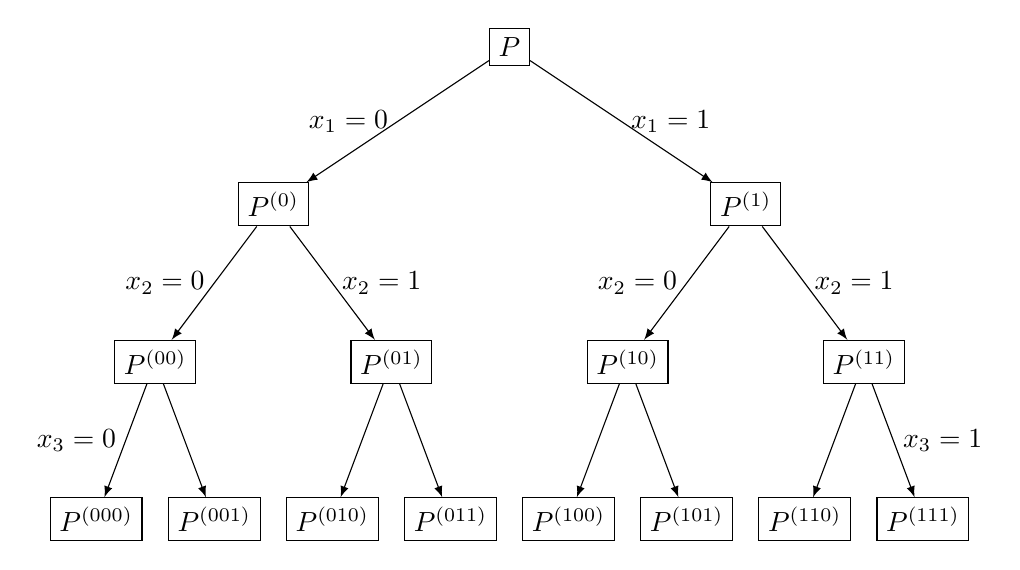
\begin{tikzpicture}[every child node/.style={rectangle,draw},level 1/.style={sibling distance=6cm},level 2/.style={sibling distance=3cm},level 3/.style={sibling distance=1.5cm}, level distance = 2cm,edge from parent/.style={draw,-latex}]
        \node[rectangle,draw] (X) {$P$} 
	    child { node {$P^{(0)}$}
        	child { node {$P^{(00)}$}
		    child { node {$P^{(000)}$} edge from parent node [midway,left] {$x_3=0$} }
		    child { node {$P^{(001)}$} }
		    edge from parent node [midway,left] {$x_2=0$}
		}
        	child { node {$P^{(01)}$}
		    child { node {$P^{(010)}$} }
		    child { node {$P^{(011)}$} }
		    edge from parent node [midway,right] {$x_2=1$}
		}
        	edge from parent node [midway,left] {$x_1=0$}
            }
            child { node {$P^{(1)}$}
        	child { node {$P^{(10)}$}
		    child { node {$P^{(100)}$} }
		    child { node {$P^{(101)}$} }
		    edge from parent node [midway,left] {$x_2=0$}
		}
        	child { node {$P^{(11)}$}
		    child { node {$P^{(110)}$} edge from parent }
		    child { node {$P^{(111)}$} edge from parent node [midway,right] {$x_3=1$} }
		    edge from parent node [midway,right] {$x_2=1$}
		}
        	edge from parent node [midway,right] {$x_1=1$}
            }
            ;
	%\node[left = of x2] (x2_label) {$x_2=$};
	%\node at (x2_label |- x1) {$x_1=$};
	% \node[left = of x1 -| x2] {$x_1=$};
    \end{tikzpicture}
    \caption{Complete decomposition of an MILP problem on its 3 binary variables. Nodes are annotated with the associated subproblems. Assuming that the problem has no other integer variables, the subproblems at the leaf nodes are LP problems.}
    \label{fig:binary-MILP-tree-example}
\end{figure}

Unfortunately, completely decomposing an MILP problem through the integer variable assignments is only possible for very small, bounded problems.
If the problem is unbounded in the integer variables, the complete decomposition would result in an infinite recursion.
Furthermore, the number of leaf nodes grows exponentially with the size of the problem\footnotemark.
\footnotetext{In this context, the size of the problem is measured as the number of binary variables that the equivalent reformulation as a binary MILP would contain. The number of leaf nodes grows exponentially (with base 2) with respect to the number of such binary variables.}

The branch-and-bound algorithm follows an implicit approach that uses upper and lower bounds to avoid indefinitely dividing subsets from the decomposition.
Let $P$ be an MILP problem formulated as in \eqref{eq:general-milp} and $X_1,\ldots,X_K$ be a decomposition of the feasible region $X$.
If $\underline{z}^{k}$ and $\overline{z}^{k}$ are lower and upper bounds to $z^{k}$ (optimum cost of $P^{(k)}$), for every $k=1,\ldots,K$, then, it is true that \[
\min_k \underline{z}^{k} \le z \le \min_k \overline{z}^{k}
,\] 
where $z$ is the optimum cost of $P$.
In other words, we can compute bounds of the root problem as $\underline{z}\gets \min_k \underline{z}^{k}$ and $\overline{z}\gets \min_k \overline{z}^{k}$.
Finally, if $\underline{z}^{k} \ge \overline{z}$ for a given $k$, then the optimal solution of $P^{(k)}$ will not be an optimal solution of $P$, because it is guaranteed that another subproblem has a better feasible solution.
In other words, even if the optimal solution of $P^{(k)}$ is unknown, it is possible to disregard $X_k$ in the decomposition, i.e., $X_k$ does not need to be further subdivided. 

For example, let $P$ be an MILP problem and $X=X_1\cup X_2$ be a decomposition such that $X_1=\{\bm{x}\in X: x_1 \le 2\}$ and $X_2=\{\bm{x}\in X: x_1 \ge 3\}$.
Suppose that the LP relaxations\footnote{The linear programming problem obtained by ignoring the integrality constraints of an MILP is called its \emph{LP relaxation}.} of $P^{(1)}$ and $P^{(2)}$ were solved to optimality, giving lower bounds $\underline{z}^1=20$ and $\underline{z}^{2}=15$, and that a feasible solution to $P$ is known in $X_2$ such that the upper bound $\overline{z}^{2}=17$ is known.
Fig.~\ref{fig:pruning-example-milp} illustrates the decomposition along with respective bounds in the form of a tree.
Because the lower bound of $P^{(1)}$ is greater than the original problem's upper bound (as $\overline{z}=\min_k \overline{z}^{k}$), the optimal solution is definitely not in $X_1$, so this set is ignored in the decomposition and not further refined.

\begin{figure}[h]
    \centering
    \begin{tikzpicture}[every child node/.style={rectangle,draw},level 1/.style={sibling distance=3cm}, level distance = 2cm,edge from parent/.style={draw,-latex}]
        \node[rectangle,draw] (P) {$P$} 
	    child { node[fill=red!50] (P1) {$P^{(1)}$}
        	edge from parent node [midway,left] (x1) {$x_1\le 2$}
            }
            child { node (P2) {$P^{(2)}$}
        	edge from parent node [midway,right] {$x_1 \ge 3$}
            }
            ;
	%\node[above = 0cm of P] {$15\le z\le 17$} ;
	\node[right = 0.5cm of P.south] {$15$} ;
	\node[right = 0.5cm of P.north] {$17$} ;
	\node[right = 0.5cm of P1.south] {$20$} ;
	\node[right = 0.5cm of P2.north] {$17$} ;
	\node[right = 0.5cm of P2.south] {$15$} ;
	%\node[left = of x2] (x2_label) {$x_2=$};
	%\node at (x2_label |- x1) {$x_1=$};
	% \node[left = of x1 -| x2] {$x_1=$};
    \end{tikzpicture}
    \caption{Example of pruning the decomposition of an MILP problem based on known bounds. The lower (resp. upper) bounds of each (sub)problem are annotated at the bottom (resp. top) right of each node. The node associated to set $X_1$ is painted red to indicate it is pruned based on the bounds of the root problem, which are updated based on the bounds from $P^{(2)}$.}
    \label{fig:pruning-example-milp}
\end{figure}

Because of the usual tree representation, the operation of disregarding a set in the decomposition is often called \emph{pruning}.
Three basic rules can be listed that lead to pruning of the branch associated to set $X_k$:
\begin{itemize}
    \item[Optimality] Subproblem $P^{(k)}$ was solved to optimality (e.g., through its LP relaxation having an optimal solution that respects the integrality constraints);
    \item[Bound] The associated lower bound is higher than the upper bound of the root problem ($\underline{z}^{k}\ge \overline{z}$);
    \item[Infeasibility] $X_k = \varnothing$.
\end{itemize}


The two key components of a branch-and-bound algorithm are the pruning system based on \emph{bounds}, as discussed above, and the rules for subdividing the sets in the decomposition, or \emph{branching}.
A simple strategy for branching is to choose an integer variable that has taken a fractional value in the optimal solution to the LP relaxation and split the problem on this factional value.
For example, let $X_k$ be a set in the decomposition of an MILP problem, and $P^{(k)}$ be the associated subproblem.
Let $\widetilde{\bm{x}}^{k}$ be the solution to the LP relaxation of $P^{(k)}$, and suppose that the integer variable $x_3$ takes value $3.67$ in $\widetilde{\bm{x}}^{k}$.
Following the proposed branching strategy on $x_3$, the sets $X_{k_1}$ and $X_{k_2}$ would be created such that \[
X_{k_1} = \left\{ \bm{x} \in X_k : x_3 \le 3 \right\} ,\, X_{k_2} = \left\{ \bm{x}\in X_k : x_3 \ge 4 \right\} 
,\] and the set $X_k$ would then be replaced in the decomposition by these two new sets.
Fig.~\ref{fig:branching-example} illustrates this example.

\begin{figure}[h]
    \centering
    \begin{tikzpicture}[every child node/.style={rectangle,draw},level 1/.style={sibling distance=3cm}, level distance = 2cm,edge from parent/.style={draw,-latex}]
        \node (P) {} 
	    child { node[draw=none] (P1) {}
        	edge from parent [draw=none]
            }
            child { node (Pk) {$P^{(k)}$}
		child { node [solid] (Pk1) {$P^{(k_1)}$}
		    edge from parent [solid] node [midway,left] (x1) {$x_3\le 3$}
		}
		child { node [solid] (Pk2) {$P^{(k_2)}$}
		    edge from parent [solid] node [midway,right] (x2) {$x_3\ge 4$}
		}
        	edge from parent [dashed] 
            }
            ;
	\node[right = 0cm of Pk.east] {$\widetilde{x}^{k}_3 = 3.67$} ;
    \end{tikzpicture}
    \caption{Example of branching on a given set $X_k$ which is part of the decomposition of an MILP problem. Only the relevant part of the tree is illustrated (indicated by the dashed arrow). The optimum value of $x_3$ (the selected integer variable for branching) in the LP relaxation of $P^{(k)}$ is annotated next to the appropriated node.}
    \label{fig:branching-example}
\end{figure}

Note that by branching on the fractional value of an integer variable in the optimal solution to the LP relaxation, the optimal solution of the LP relaxation becomes infeasible in the LP relaxations of the new sets\footnote{This is true unless there are degeneracies such as multiple solutions in the LP relaxation}.
Therefore, after branching, the best lower bound will necessarily increase.
Using the example above to make this result tangible, it is possible to state that $\widetilde{\bm{x}}^{k}$ is infeasible for the LP relaxations of both $P^{(k_1)}$ and $P^{(k_2)}$.
Therefore, $\max\{\underline{z}^{k_1},\underline{z}^{k_2}\} > \underline{z}^{k}$.

%As an example, take the MILP problem\footnote{Example taken from \citeonline{vanderbeiLinearProgrammingFoundations1998}, Ch. 22.5.}
%\begin{align*}
%    \min_{\bm{x}} \quad & -17 x_1 - 12x_2 \\
%    \textrm{s.t.} \quad & 10x_1 + 7x_2 \le 40 \\
%      & x_1+x_2\le 5 \\
%      & \bm{x} \in \Z_+^2
%.\end{align*}

There are many more intricate details to the construction of a branch-and-bound algorithm, such as the strategy for choosing a set in the decomposition to refine, the amount of information from each node of the tree to be stored, efficient reoptimization, and computing the bounds using the dual.
The reader is pointed to \citeonline{wolseyIntegerProgramming1998} and \citeonline{vanderbeiLinearProgrammingFoundations1998} for advanced topics and detailed examples.


\subsection{Heuristics}

Although branch-and-bound provides an efficient algorithmic approach to solve an MILP problem, there is no guarantee that it will find a feasible (let alone an optimal) solution considering the NP-hardness of the problem.
The development of heuristic or approximation algorithms is justified in many ways, as can be seen in \citeonline{wolseyIntegerProgramming1998}, Chapter 12.
The major one, for this work, is from practical applications with significant running time cost.
In simple terms, such applications require good solutions quickly, rather than optimal solutions in an unknown time-horizon.

Heuristic algorithms are an umbrella term that encompass several different algorithms with different characteristics.
Overall, distinguishing features of heuristics are on the feasibility and optimality of the solutions returned.
For feasibility, it is important to know if there are feasibility guarantees on the heuristic solution or, at least, an expectation on how often the heuristic will return infeasible solutions.
Similarly, it is relevant to understand whether the solutions provided are guaranteed to be within a limited distance (in terms of the objective function) of the optimal solutions, or if there is an expected value for such distance. 
Such heuristics with quality guarantees are referred to as approximation algorithms in the technical literature

Common examples of heuristic algorithms are greedy algorithms and local search approaches~\cite{nemhauserIntegerCombinatorialOptimization1999,wolseyIntegerProgramming1998}.
Greedy heuristics construct the solution incrementally by selecting, at each step, the alternative that best improves the objective function.
Take the Symmetric TSP (STSP) as an example.
A greedy heuristic for such problem could be to add to the solution the edge with the smallest cost.
Note that this greedy heuristic will always return a feasible solution, although it is not expected that the solution will be close to optimal.

Local search algorithms take a feasible solution and try to improve the objective function by performing only limited changes.
Given a complete tour (feasible solution) for the STSP, a small deviation can be achieved by removing two non-consecutive edges that are part of the solution and adding two \emph{different} edges that reconnect the two disjoint paths.
This way, a new tour will be achieved that differs from the original by two edges.
In other words, such local search is limited to a 2-neighborhood of the original tour.

A general heuristic (or metaheuristic) algorithm for MILP problems is \emph{diving}~\cite{fischettiHeuristicsMixedInteger2011}.
Diving methods solve the LP relaxation, fix integer variables that assume fractional values, and update the LP relaxation.
This process is repeated until there are no more integer variables to be fixed.
It is often called diving because it is equivalent to quickly navigating to a leaf node in a branch-and-bound tree.

Recently, heuristics based on machine learning models have been proposed~\cite{bengioMachineLearningCombinatorial2021}.
This will be discussed in Section~\ref{sec:learning-based-heuristics}.

\subsubsection{Matheuristics}

Matheuristics is the name given to heuristic algorithms that use a mathematical programming model at its core.
In fact, the diving algorithm introduced above can be seen as a form of matheuristic.
In this section, however, the focus is on algorithms that actively optimize mathematical programming models.
Relaxation induced neighborhood search (RINS)~\cite{maniezzoMatheuristicsAlgorithmsImplementations2021} exemplifies the distinction intended in this chapter.

The RINS algorithm aims to improve a feasible solution by solving a smaller MILP problem. 
A neighborhood around a feasible solution is defined by fixing the values of some integer variables.
The search on this neighborhood is performed by adding the variable fixing constraints to the original problem, effectively reducing its feasible region.
Let $P$ be an MILP problem as in \eqref{eq:general-milp}, $\bm{x}^{h}$ be a feasible solution, and $\widetilde{\bm{x}}$ the solution to the LP relaxation of $P$.
Let $J = \{j = 1,\ldots,n : x_j^{h} = \widetilde{x}_j\}$ be the index set of \textcolor{blue}{integer} variables to fix.
Then, the sub-MILP problem
\begin{align*}
    \min_{\bm{x}} \quad & \bm{c}^{T}\bm{x} \\
    \textrm{s.t.} \quad & A\bm{x}\le \bm{b} \\
      & x_j = x_j^{h}, \forall j \in J \\
      & \bm{x}\in \Z^{n}\times \R^{p}
\end{align*}
can be solved, e.g., using branch-and-bound.
Note that all integer variables that assume the same value in the feasible solution and in the solution to the LP relaxation are fixed, thus, reducing the search space, but abdicating from optimality guarantees.

As the RINS example above illustrates, a mathematical programming model plays a central role in a matheuristic~\cite{fischettiMatheuristics2016}.
Because of their flexibility, matheuristics are also used within branch-and-bound algorithms, e.g., to find tighter bounds and accelerate the time to reach the first feasible solution~\cite{fischettiMatheuristics2016,maniezzoMatheuristicsAlgorithmsImplementations2021}.

\subsubsection{Performance analysis}

The performance analysis of heuristic algorithms depends on the instances of interest.
To better formalize this idea, let us write
\begin{align*}
    P(I): \min_{\bm{x}} \quad & \bm{c}_I^{T}\bm{x} \\
    \textrm{s.t.} \quad & A_I\bm{x} \le \bm{b}_I \\
      & \bm{x}\in \Z^{n_I}\times \R^{p_I}
,\end{align*}
for all instances $I\in \mathcal{I}$.
The set $\mathcal{I}$ contains all instances of the MILP problem of interest, e.g., all TSPs, TSPs within a given country with all possible edge weights, course scheduling for a given university for varying student interest, or energy system optimization problems for a multi-modal power plant under different weather conditions.
Using this notation, it is possible to say that the performance of the heuristic can be analyzed from the set $\mathcal{I}$.

A possible evaluation is to perform a worst-case analysis of the heuristic.
The essential idea of a worst-case analysis is to determine the maximum deviation between the optimum objective value and the objective value of the heuristic solution. 
Let $z(I)$ be the optimum objective value of instance $I\in \mathcal{I}$, and $z_H(I)$ be the objective value of the solution provided by a heuristic $H$.
The worst-case performance is, then,
\begin{equation}
    \begin{split}
	\max_{I\in \mathcal{I}} \quad& |z(I) - z_H(I)| \\
	\textrm{s.t.} \quad& X_I \neq \varnothing
    ,\end{split}
\end{equation}
where $X_I$ is the feasible region of instance $I$.

Not always, however, the worst-case performance can be determined analytically.
A performance estimate can be defined in such cases.
Let $\mathcal{P}$ be a probability distribution over $\mathcal{I}$.
The expected performance of a heuristic can be defined as \[
    \mathbb{E}_{I\sim \mathcal{P}} |z(I) - z_H(I)|
,\] which can be approximated by Monte Carlo sampling.



